
\begin{figure}[h]
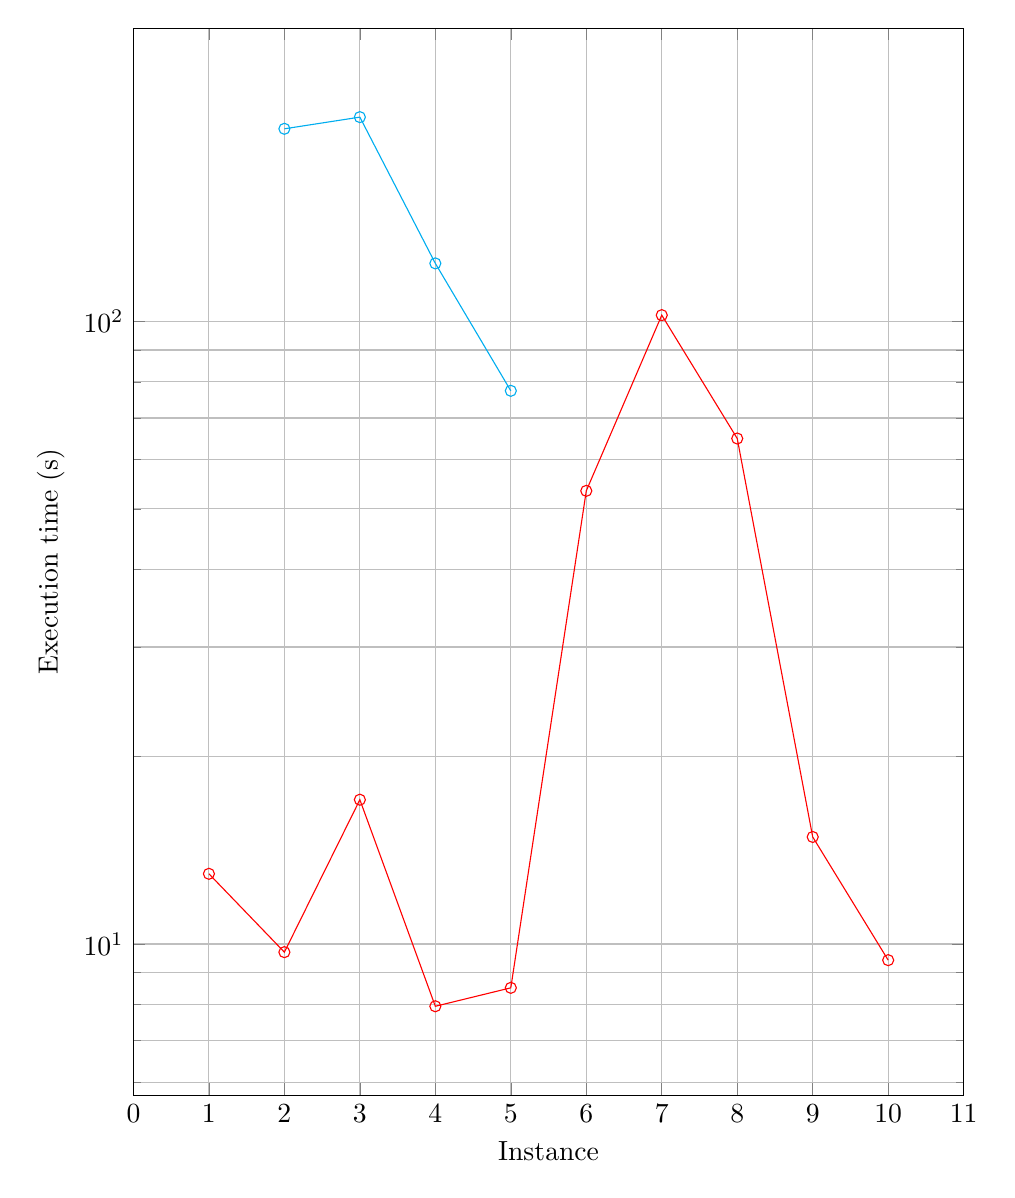
\begin{tikzpicture}
	\begin{axis}[width=\textwidth,height=100ex,
		xlabel=Instance,
		ylabel=Execution time (s), xmin=0, ymin=0, grid=both,
		ymode=log]

% gurobi p3
\addplot[mark=o,color=red] coordinates {
(1, 12.96708331)
(2, 9.704563172)
(3, 17.056811547)
(4, 7.944795782)
(5, 8.505190252)
(6, 53.456992427)
(7, 102.392618933)
(8, 64.881486922)
(9, 14.86064378)
(10, 9.421963416)
};

% cbc nothing - too slow
\addplot[mark=o,color=green] coordinates {
};

% cbc with random heuristic
\addplot[mark=o,color=cyan] coordinates {
(2, 204)
(3, 213)
(4, 124)
(5, 77.41492818)
%
%
%

};

% cbc with ff heuristic
\addplot[mark=o,color=brown] coordinates {
};

% cbc with divisor 100 - too slow
\addplot[mark=o,color=purple] coordinates {};

\end{axis}

\end{tikzpicture}%
\caption{Execution time for all relevant cases using P3. Red: Gurobi, cyan: Cbc using the random heuristic, brown: Cbc using the farthest-first heuristic}
\end{figure}
